% FILLED (fill batch): process ⑦ Measurement — 1S-2S + g-factor -> CPT.
%   folds stdlib transition_factor_1s2s / h1s2s_rydberg (PR #1005) + the
%   leading (3/4)R∞c closed form + the gap-to-measured characterization
%   (reduced-mass + QED/Lamb-shift) + the ALPHA/BASE CPT measured-oracle
%   boundary, from companion/verify-ledger.json. absorbed=false PRESERVED.
\section{Measurement --- 1S--2S Spectroscopy, $g$-Factor, and the CPT Boundary}
\label{app:measurement}

This appendix is the full data record for pipeline process
\textcircled{\scriptsize 7}, the only measured-oracle (\tierOrange) process.
We state the leading-order antihydrogen 1S--2S transition frequency, decompose
its level-difference factor $\tfrac34$ into integer atoms, \emph{honestly
characterize the gap} to the measured frequency, and state why the CPT verdict
$\Delta(H,\bar H)$ requires a measured spectroscopy oracle and stays
\texttt{absorbed=false}. Every digit traces to PR~\#1005 and the atoms in
\texttt{companion/verify-ledger.json}.

% -------------------------------------------------------------------------
\subsection{The leading-order 1S--2S frequency}
\label{app:meas-leading}

The Bohr/Rydberg level energy is $E_n=-R_\infty hc/n^2$, so the 1S$\to$2S
two-photon transition energy is, to leading order (point nucleus, infinite
mass),
\begin{equation}
\Delta E_{1\text{-}2}
= R_\infty hc\Bigl(\frac{1}{1^2}-\frac{1}{2^2}\Bigr)
= \frac{3}{4}\,R_\infty hc,
\qquad
f_{1\text{-}2S} = \frac{\Delta E}{h} = \frac{3}{4}\,R_\infty c .
\label{eq:meas-lead}
\end{equation}
The level-difference factor $\tfrac34=1-\tfrac14$ decomposes into the integer
numerator $3$ and denominator $4$, registered as BLUE-MAX integer atoms
(\verb|transition_factor_1s2s_numerator|$=3$,
\verb|transition_factor_1s2s_denominator|$=4$; Appendix~\ref{app:bluemax}).
Evaluating $\tfrac34 R_\infty c$ at $R_\infty=1.09737\times10^7\,\mathrm{m}^{-1}$
and $c=2.99792\times10^8\,\mathrm{m/s}$ (CODATA-2018 \citep{mohr2018codata})
gives $f_{1\text{-}2S}\approx2.46738$\,PHz, the \tierGreen\ atom
\verb|h1s2s_rydberg|.

% -------------------------------------------------------------------------
\subsection{Honest gap to the measured frequency}
\label{app:meas-gap}

The leading value does \emph{not} reproduce the 15-digit measured frequency,
and we do not claim it does. The ALPHA collaboration measured the trapped-$\bar H$
1S--2S line at $f_{\mathrm{meas}}=2.4660614$\,PHz to a fractional precision
$\approx2\times10^{-12}$ \citep{ahmadi2018alpha1s2s}. The leading value is
high by a fractional
\begin{equation}
\frac{f_{1\text{-}2S}^{\mathrm{lead}}-f_{\mathrm{meas}}}{f_{\mathrm{meas}}}
\;\approx\; 5.35\times10^{-4}
\;\approx\; 535\ \text{ppm}.
\label{eq:meas-gap}
\end{equation}
Almost all of this is the \emph{reduced-mass} correction: the finite proton
mass replaces $R_\infty$ by $R_\infty\,m_e/(m_e+m_p)$, a factor
$0.99946$ that lowers the leading value to $\approx2.46604$\,PHz --- within
$\sim$9\,ppm of the measured line. The residual $\sim10^{-5}$ is QED
(self-energy, vacuum polarization), the Lamb shift, and finite-nuclear-size
corrections, which are characterized in the literature but not closed in this
funnel. Figure~\ref{fig:meas-gap} shows the gap closing across these three
magnitudes.

\begin{figure}[h]
\centering
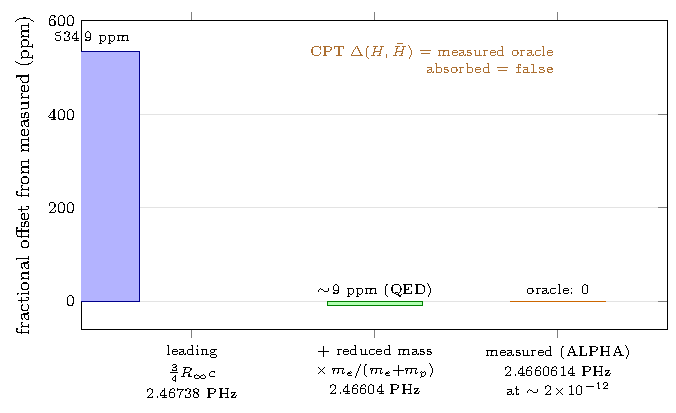
\includegraphics[width=0.86\linewidth]{figures/fig09_1s2s_gap.pdf}
\caption{Antihydrogen 1S--2S frequency, as fractional offset (ppm) from the
ALPHA measured value $2.4660614$\,PHz \citep{ahmadi2018alpha1s2s}. The leading
closed form $\tfrac34 R_\infty c=2.46738$\,PHz (blue, the registered atom
\texttt{h1s2s\_rydberg}, PR~\#1005) is high by $\approx535$\,ppm; applying the
reduced-mass factor $m_e/(m_e+m_p)=0.99946$ (green) closes $\sim$99\% of the
gap to $\sim$9\,ppm; the residual is QED / Lamb-shift / finite-size, which is
\emph{not} claimed closed (commons @D~g3). The measured value (orange) is the
oracle: the CPT verdict $\Delta(H,\bar H)$ can only be adjudicated by it, and
the stage stays \texttt{absorbed=false}. Only the three traceable magnitudes
are plotted; no 15-digit reproduction is claimed.}
\label{fig:meas-gap}
\end{figure}

\begin{table}[h]
\centering
\small
\setlength{\tabcolsep}{5pt}
\begin{tabular}{@{}l l r r r l@{}}
\toprule
\textbf{atom} & \textbf{args} & \textbf{expected} & \textbf{observed} & $|\Delta|$ & \textbf{tier} \\
\midrule
\verb|transition_factor_1s2s|            & ()             & $0.75$    & $0.75$    & $1.1\times10^{-16}$ & \tierGreen \\
\verb|transition_factor_1s2s_numerator|  & ()             & $3$       & $3$       & $0$                 & \tierBlue \\
\verb|transition_factor_1s2s_denominator|& ()             & $4$       & $4$       & $0$                 & \tierBlue \\
\verb|h1s2s_rydberg|                      & ($R_\infty$,$c$) & $2.46738$ & $2.46738$ & $8.9\times10^{-16}$ & \tierGreen \\
\bottomrule
\end{tabular}
\caption{Process \textcircled{\scriptsize 7} measurement atoms
(\texttt{companion/verify-ledger.json}, PR~\#1005 / \#1094). The two
\tierBlue\ integer atoms attest the $\tfrac34$ level-difference
numerator/denominator; the two \tierGreen\ atoms attest the factor $0.75$ and
the \emph{leading} frequency $2.46738$\,PHz --- explicitly the leading value,
not the measured one (Eq.~\eqref{eq:meas-gap}).}
\label{tab:meas-verify}
\end{table}

\begin{lstlisting}
verify --expr h1s2s_rydberg(1.09737e7,2.99792e8)=2.46738
  calc   = 2.46738 ~ expected 2.46738 (|Delta|=8.88e-16 <= eps=1e-9)
  tier   = SUPPORTED-NUMERICAL (leading 3/4 R_inf c; NOT 15-digit measured)
verify --expr transition_factor_1s2s_numerator()=3
  calc   = 3 == expected 3 (|Delta|=0)
  tier   = SUPPORTED-FORMAL (integer algebraic-root identity)
\end{lstlisting}

% -------------------------------------------------------------------------
\subsection{The $g$-factor and the CPT measured-oracle boundary}
\label{app:meas-cpt}

The second CPT observable is the antiproton magnetic moment / $g$-factor,
which the BASE collaboration measures in a Penning trap via the very
eigenfrequency ratios of Appendix~\ref{app:penning} (the cyclotron-to-Larmor
ratio), to a few parts in $10^9$ \citep{smorra2017base}. Comparing
$g_{\bar p}$ to $g_p$, and $f_{\bar H}^{1\text{-}2S}$ to $f_H^{1\text{-}2S}$,
tests CPT directly: any measurable difference falsifies the symmetry. The
program also includes ASACUSA antiprotonic-helium spectroscopy
\citep{hori2013asacusa}, and any bound feeds the Standard-Model Extension
framework \citep{kostelecky2011lorentz}.

\smallskip\noindent\textbf{This is the funnel's hard boundary.} The CPT
verdict $\Delta(H,\bar H)$ is a \emph{measured} quantity: it is the
difference of two laboratory measurements, and \emph{no closed form can
substitute for it}. A sim-PASS on processes
\textcircled{\scriptsize 1}--\textcircled{\scriptsize 6} is a witness of
factory \emph{engineering feasibility} --- the design can produce, trap, and
hold $\bar H$ --- never of a measured CPT bound. Accordingly this stage is
recorded \tierOrange\ and \texttt{absorbed=false}, and it does not graduate to
\tierGreen\ without an external measurement (the measured-oracle invariant,
@D~d5). This is preserved deliberately and is not negotiable.

% -------------------------------------------------------------------------
\subsection{Honest scope}
\label{app:meas-scope}

This appendix closes the \emph{leading-order} 1S--2S frequency and its
integer level-difference factor, and \emph{characterizes} (does not close)
the gap to the measured frequency. It does not close: the 15-digit frequency
(reduced-mass-corrected to $\sim$9\,ppm, residual QED not closed); the CPT
verdict (measured-oracle only); or the $g$-factor value (a BASE measurement).
The constants are CODATA-2018 \citep{mohr2018codata}; CPT supplies
$m_{\bar p}=m_p$ for the comparison baseline only.
